\chapter{Method}

% \section{Voxelnet}
% VoxelNet is an End-to-End Learning for Point Cloud Based 3D Object Detection. The work is described in Yin Zhou and Oncel Tuzel's paper: \cite{https://doi.org/10.48550/arxiv.1711.06396}.

% In order to implement this work, the following git repo is adapted: \url{https://github.com/qianguih/voxelnet}. This repo contains a pre-trained model, trained to detect cars from the velodyne lidar data provided by the KITTI dataset.

% \section{ViperX 300 Robot Arm}
% In order to operate the Trossen Robotics ViperX 300 Robotic Arm, Their ROS 2 packages are utilised.
% These can be found here: \url{https://docs.trossenrobotics.com/interbotix_xsarms_docs/}.

This chapter will describe different methodologies used to solve technical problems over the course of this project.

\section{Problem Formulation}

The objective of this project is to set up an autonomous warehouse system where an autonomous UGV should be able to fetch objects in a warehouse. The system will rely on an UGV equipped for autonomous navigation to move around in the environment. The UGV will also be equipped with a robotic manipulator for pick and place operations.

\section{Conceptual Design}
The design of the robot should reflect the intended tasks of the robotic platform. For an autonomous warehouse robot, these tasks involve autonomous navigation, pick and place and object detection/recognition. The design should deliver a platform that could be used for future projects. 

\subsection{Initial Concept}
With the described design specifications considered, the initial conceptual design resulted in the following major components:

\begin{itemize}
    \item Clearpath - Husky A200 UGV
    \item Redshift Labs - UM7 IMU
    \item Ouster -  OS1-64 3D LiDAR
    \item Universal Robots - UR5
    \item Intel - Realsense D435i Camera
    \item 2 X NVIDIA - Jetson AGX Xavier
\end{itemize}

From the bulletin list above, Husky A200, seen in figure \ref{fig:huskyA200}, provides a robust mobile platform and UM7 IMU and Ouster OS1-64 LiDAR provides sensory information to allow for autonomous navigation. The UR5 robotic manipulator, seen in figure \ref{fig:ur5}, paired with an Intel Realsense D435i, adds capabilities for pick and place operations with object detection and 6-DOF pose estimation. The two NVIDIA Jetson AGX Xaviers will be used to control the platform.

\begin{figure}[H]
  \centering
  \begin{minipage}[b]{0.49\textwidth}
        \centering
        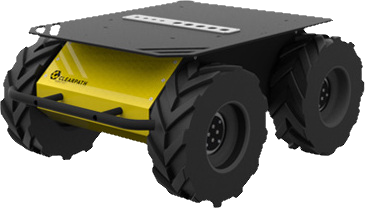
\includegraphics[width = 0.8\textwidth]{Figures/huskyA200.png}
        \caption{Clearpath Husky A200. Image adapted from \cite{clearpath_husky_website}}
        \label{fig:huskyA200}
  \end{minipage}
  \hfill
  \begin{minipage}[b]{0.49\textwidth}
    \centering
    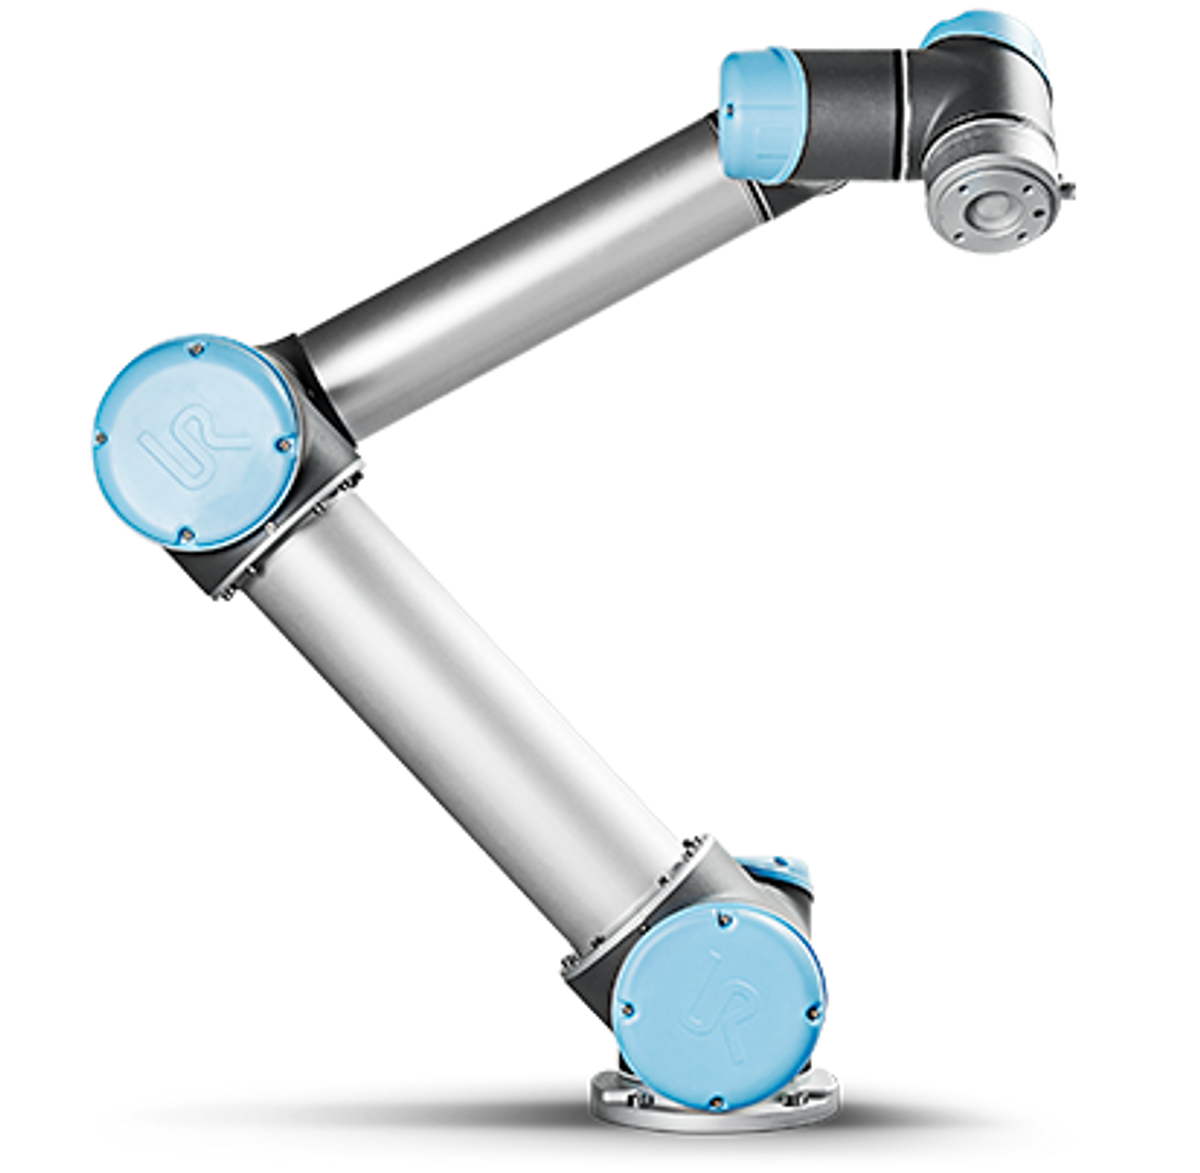
\includegraphics[width = 0.8\textwidth]{Figures/ur5.png}
    \caption{Universal Robots UR5. Image from \cite{ur5_img}}
    \label{fig:ur5}
  \end{minipage}
\end{figure}

Some specifications on the Husky A200 robotic platform is listed in table \ref{tab:husky:a200:specs}

\begin{table}[H]
\centering
\caption{Technical specifications for the Clearpath Husky A200, complete data sheet available in appendix \ref{A:fig:husky_data_sheet}, from \cite{clearpath_husky_website}}
\label{tab:husky:a200:specs}
\vspace{1mm}
\begin{tabular}{ll}
\hline
\multicolumn{2}{c}{\textbf{Husky A200 Specifications}}                                                            \\ \hline
Drivers and APIs                            & ROS, ROS 2, C++ and Python                                          \\
Wheel encoders                              & Quadrature: 78,000 {[}pulses/m{]}
        \\
Communication                               & RS232@115200 Baud                                                   \\
Battery                                     & \begin{tabular}[c]{@{}l@{}}12V 20Ah\\ Sealed Lead Acid\end{tabular} \\
\multicolumn{1}{c}{User Power Distribution} & \begin{tabular}[c]{@{}l@{}}5V 5A\\  12V 5A\\  24V 5A\end{tabular}   \\
Weight                                      & 50 {[}kg{]}                                                         \\
Payload Capacity                            & 75 {[}kg{]}                                                         \\
External Dimensions                         & 990 x 670 x 390 {[}mm{]}                                            \\ \hline
\end{tabular}
\end{table}

One NVIDIA Jetson AGX Xavier, hereby called "UGV Xavier", interfaces with Husky, LiDAR and IMU. This computer will control the Husky and take care of autonomous navigation tasks such as mapping, localization and path planning. 

The second NVIDIA Jetson AGX Xavier, hereby called Manipulator Xavier, interfaces with the Realsense camera and robotic manipulator. This computer will control the manipulator, and take care of sensory information from the Realsense camera. 

The relatively powerful GPU of the Xaviers adds capabilities to implement deep learning algorithms to do for example image- or PointCloud based object detection.

\subsection{Final Design/Concept??}

The UR5 manipulator requires a dedicated controller to operate.This controller also contains the DC-power supply for the manipulator. As the manipulator is to be mounted on an UGV, this controller has to be powered through DC-power. According to the Universal Robots CB3 battery supply installation manual \cite{ur5_battery_manual}, the UR5 could draw up to 50A at "peak conditions". Looking at table \ref{tab:husky:a200:specs}, it is clear that the built in 24V power distribution on the Husky, with a 5A circuit breaker, is insufficient.

\begin{figure}[H]
  \centering
  \begin{minipage}[b]{0.49\textwidth}
        \centering
        The design of a mobile power system for the CB3 controller and thus, the UR5 manipulator is beyond the scope of this project. The decision was therefore made to swap out the UR5 manipulator with a smaller Interbotix VX300 manipulator from Trossen Robotics, illustrated in figure \ref{fig:vx300}. This is a significantly smaller robotic arm that is powered through 12V DC-power supply with a standard 2.5mm DC barrel jack. 
  \end{minipage}
  \hfill
  \begin{minipage}[b]{0.49\textwidth}
   \centering
  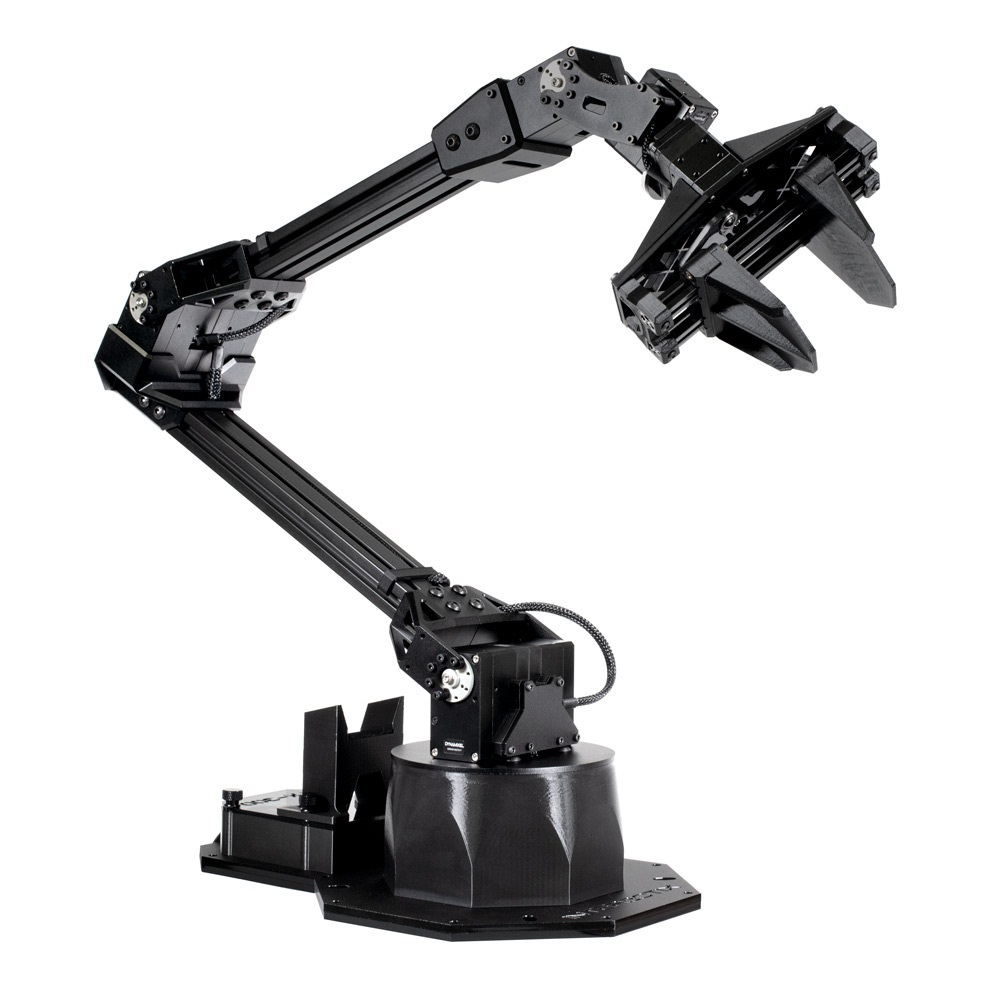
\includegraphics[width = 0.7\textwidth]{Figures/VX300.jpg}
  \caption{Interbotix Vx300. Image from \cite{interbotix_vx300}}
  \label{fig:vx300}
  \end{minipage}
\end{figure}




  
\section{Hardware}
This section describes the different hardware components of the robotic system and how they are set up for this project. A high level overview of the network topology is shown in figure \ref{fig:topology}. This topology gives an insight to how the different components are connected to create a complete system. Looking at figure \ref{fig:topology}, it can be seen that the UGV Xavier communicates with the Husky through RS232 and the UM7 IMU through USB. The LiDAR communicates through Ethernet via a WiFi router that, in this case acts as a switch. The LiDAR data is therefore available for all computers on the network. From figure \ref{fig:topology}, it can be seen that the Manipulator Xavier interfaces with both the Realsense camera and the manipulator through USB. 

\begin{figure}[H]
  \centering
  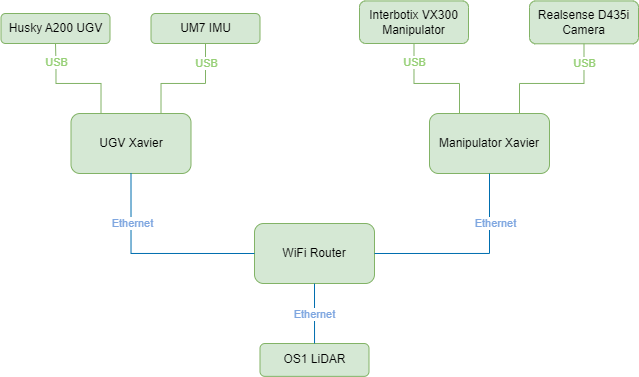
\includegraphics[width = 0.5\textwidth]{Figures/example_figure.drawio.png}
  \caption{High level network topology showing the various components on the mobile robotic platform}
  \label{fig:topology}
\end{figure}

The WiFi Router allows external computers to connect to the network, either through WiFi or cabled connection, and communicate with the two Xaviers and the LiDAR. This makes it possible to control the Xavier computers through SSH and also allows developers to interact with the ROS2 network.

\subsection{Accessory mounting frame}
As the UGV is to be used for prototyping and testing, it is preferable to have some kind of bracket where various sensors and actuators could be mounted. The bracket should be rigid, yet flexible in terms of mounting possibilities. An aluminium profile frame is therefore designed for the UGV.

\begin{figure}[H]
  \centering
  \begin{minipage}[b]{0.49\textwidth}
        \centering
         The aluminium frame, seen in figure \ref{fig:user_frame} is made out of 20X20mm aluminium profiles. The purpose of the frame is to add the possibility to mount whatever accessory the developer wants to the UGV. The choice fell on 20X20mm aluminium profiles as they are practical for mounting various equipment as well as the fact that the Husky A200 UGV is delivered with a 20x20mm mounting frame out of the box. Looking at figure \ref{fig:user_frame}, the husky mounting frame can be seen as the rectangular black frame on top of the Husky UGV.
  \end{minipage}
  \hfill
  \begin{minipage}[b]{0.49\textwidth}
   \centering
    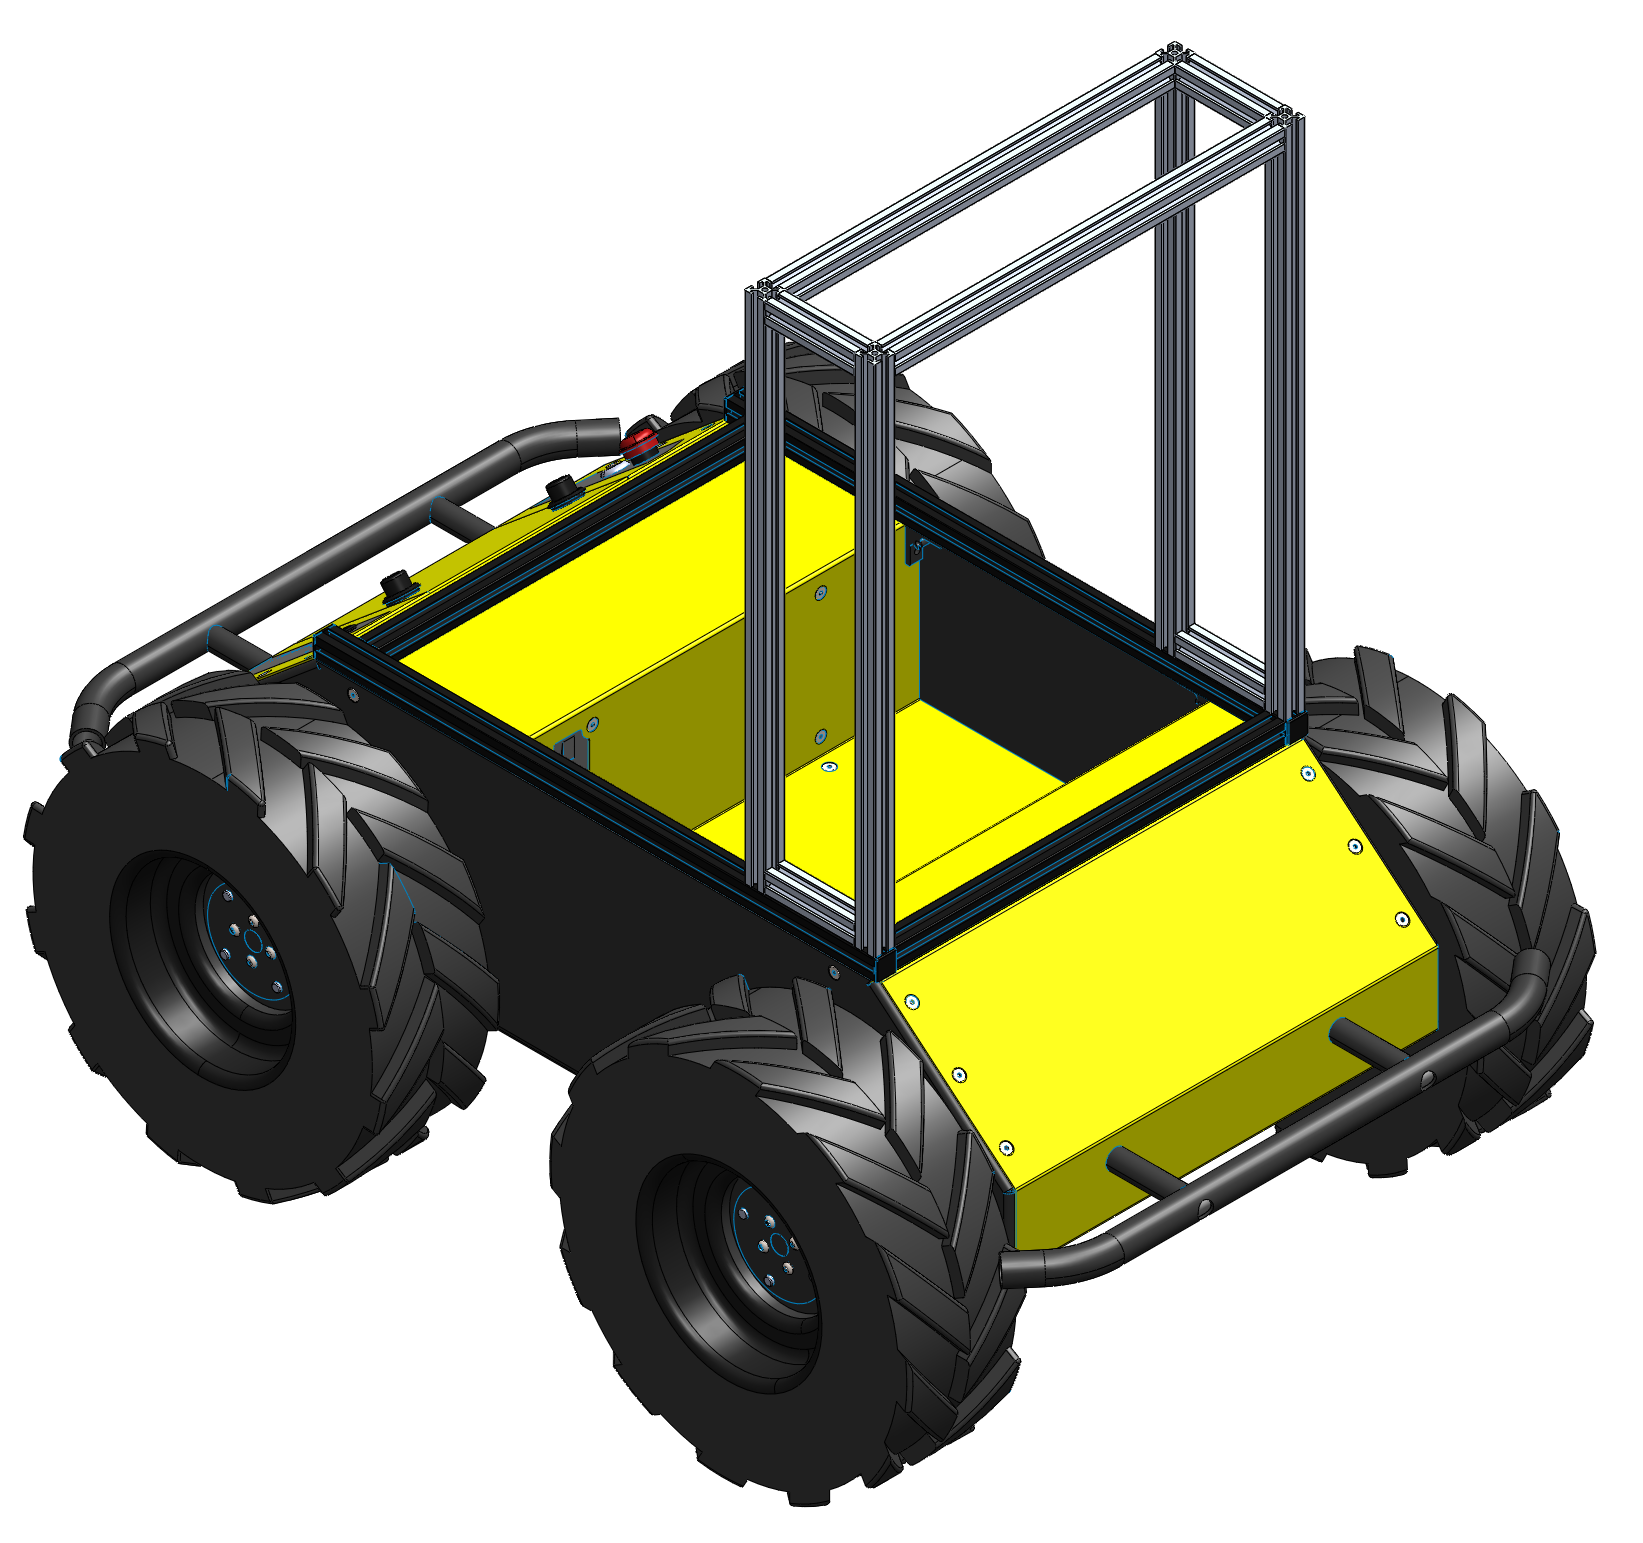
\includegraphics[width = 0.8\textwidth]{Figures/husky_with_frame.png}
    \caption{Husky A200 with sensor frame mounted}
    \label{fig:user_frame}
  \end{minipage}
\end{figure}

\subsection{Autonomous Navigation Hardware}

\subsubsection{IMU}
In order to increase the performance of the UGV odometry, an UM7 IMU from Redshift Labs, seen in figure \ref{fig:um7_imu}, has been added. This IMU is ROS2 compatible and will publish IMU data to ROS2. This data can then be used to better calculate the position of the UGV. 

\begin{figure}[H]
  \centering
  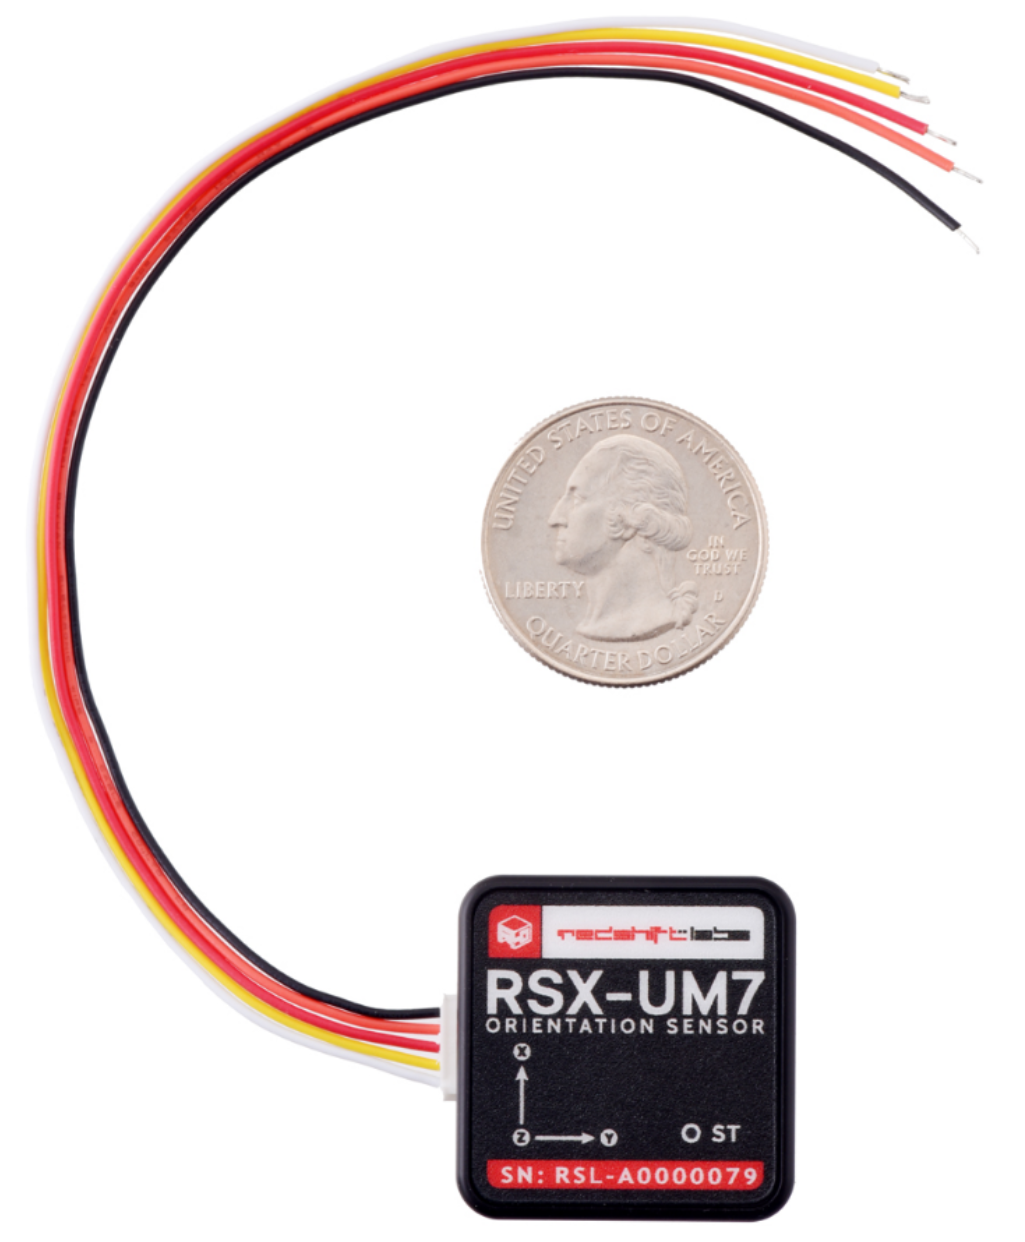
\includegraphics[width = 0.3\textwidth]{Figures/um7_imu.png}
  \caption{Redshift Labs UM7 IMU. Image from \cite{um7_imu}.}
  \label{fig:um7_imu}
\end{figure}

As illustrated in the topology in figure \ref{fig:topology}, the UM7 is connected to the UGV Xavier through USB which is used for power and communication.

\subsubsection{LiDAR}
The Ouster OS1-64, is a $360\deg$ 3D LiDAR that generates a large amount of spatial information about the surrounding environment as a point cloud. In this project, that point cloud is used for localisation and to generate a 2D map of the environment. The OS1-164 LiDAR is fitted with a built in IMU sensor which for example can be used the same way, or together with, the UM7 IMU for localisation. The LiDAR can be seen mounted on a camera bracket in figure \ref{fig:lidar_mount}.

\subsubsection{LiDAR and Camera Mount}
To account for the possibility to fuse LiDAR and image data, a LiDAR and camera mount, seen in figure \ref{fig:lidar_mount}, is created. The mount is designed to have the Ouster OS1 LiDAR mounted on the top and four e-con cameras inside. The e-con cameras are arranged $90\deg$ away from each other with a constant radius from the center of the mount.

\begin{figure}[H]
  \centering
  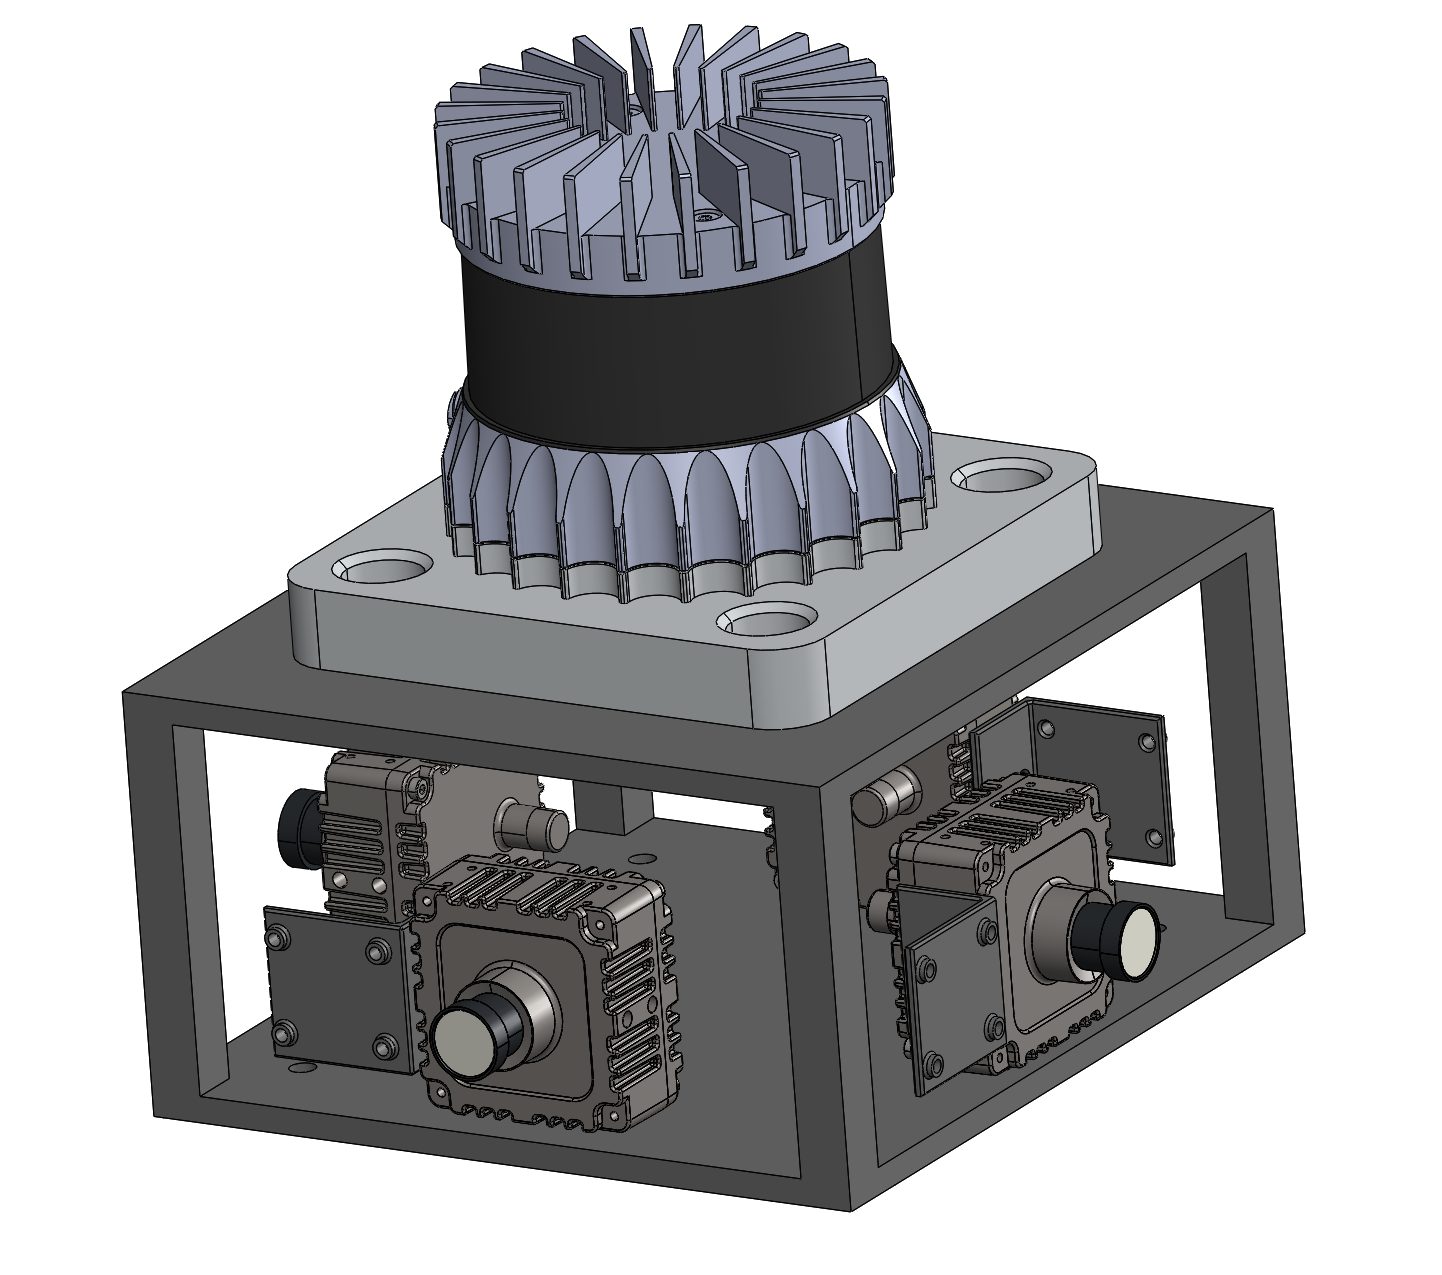
\includegraphics[width = 0.5\textwidth]{Figures/lidar_mount.png}
  \caption{Cad model of LiDAR mount with cameras. The Ouster OS1-64 is mounted on top.}
  \label{fig:lidar_mount}
\end{figure}

\subsection{Pick and Place Hardware}

\subsubsection{Manipulator}
The chosen manipulator, the Interbotix VX300 (figure \ref{fig:vx300}, is mounted on the aluminium profiles at the rear right side of the UGV. Offsetting the base of the manipulator from the center of the UGV, gives a longer reach outside of the UGV's footprint. The manipulator requires 12V power through a 2.5mm barrel jack and is connected to the husky user power supply as seen in figure \ref{fig:circuit_diagram}.

\subsubsection{Manipulator Mounted Camera}
An Intel Realsense D435i camera, seen in figure \ref{fig:d435i}, is mounted on the manipulator to add the possibility of machine vision for pick and place operations. Intel Realsense D435i is a stereo-camera from Intel with 3D vision capabilities and ROS2 compatibility. In order to mount the camera to the manipulator, a bracket has been  designed in CAD software. The bracket is adapted from \cite{d435_sleeve} with modifications to be able to mount it on the gripper of the V300 manipulator. The bracket can be seen in figure \ref{fig:realsense_assembly}.

\begin{figure}[H]
  \centering
  \begin{minipage}[b]{0.49\textwidth}
    \centering
    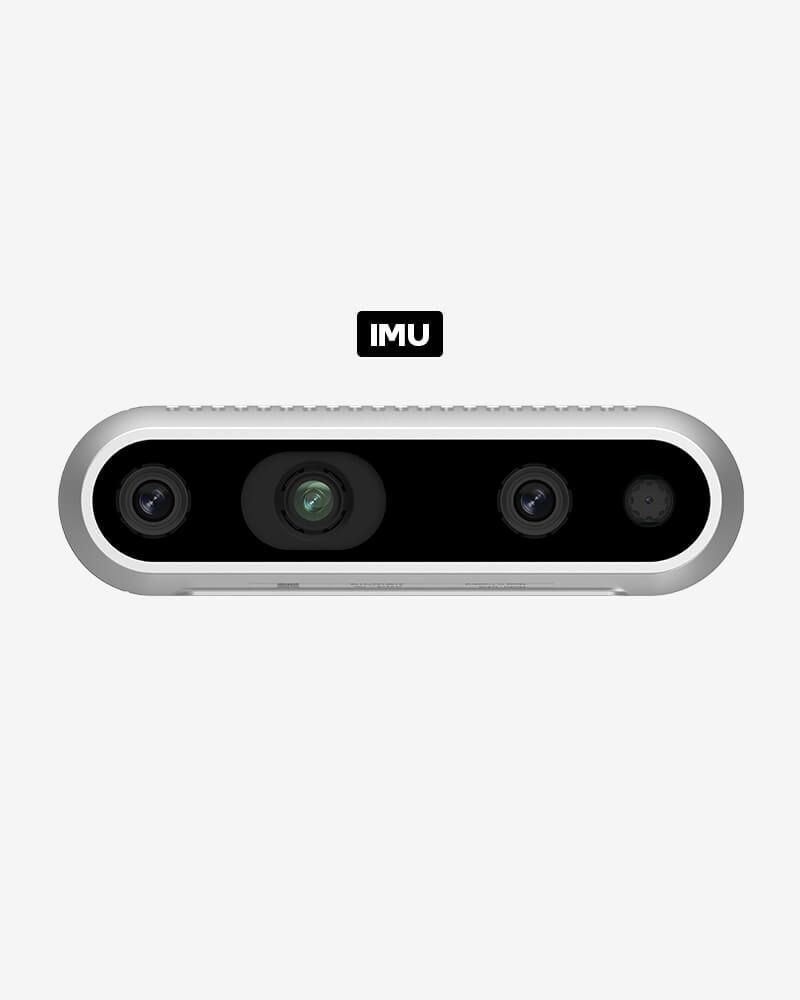
\includegraphics[width = 0.8\textwidth]{Figures/D435i.jpg}
    \caption{Intel Realsense D435i Depth Camera. Image from: \cite{realsense_d435i}.}
    \label{fig:d435i}
  \end{minipage}
  \hfill
  \begin{minipage}[b]{0.49\textwidth}
   \centering
    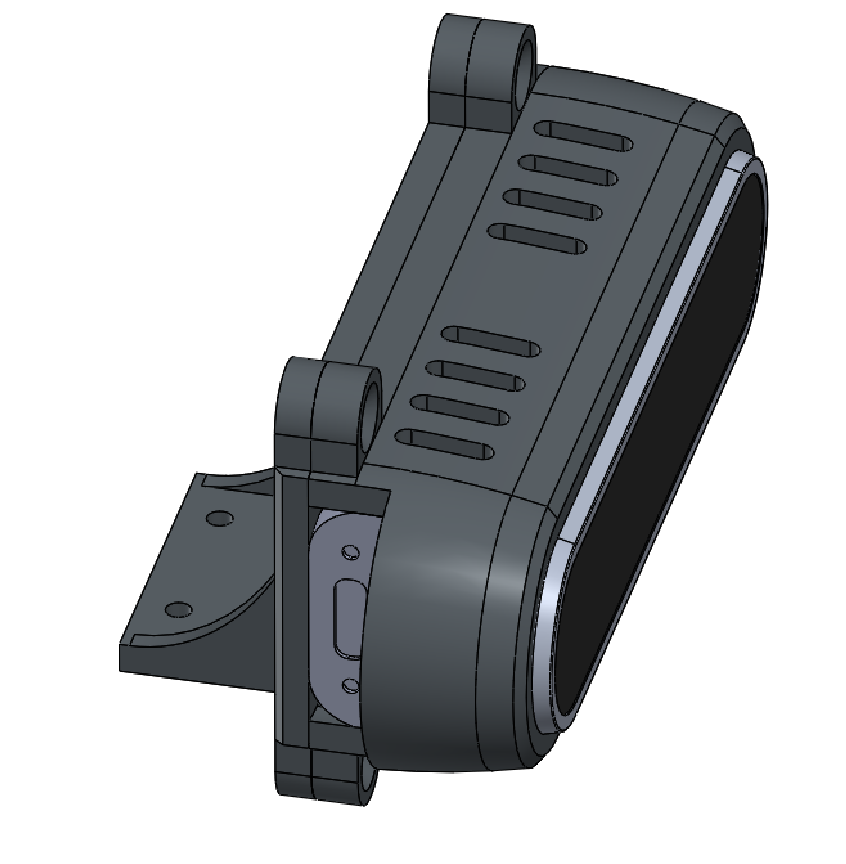
\includegraphics[width = 0.8\textwidth]{Figures/realsense_assembly.pdf}
    \caption{Realsense D435i bracket assembly with camera. The bracket is adapted from \cite{d435_sleeve} to be able to mount on the VX300 robotic arm.}
    \label{fig:realsense_assembly}
  \end{minipage}
\end{figure}

\subsection{Complete Hardware Setup}

The complete system is presented in figure \ref{fig:hardware}.

\begin{figure}[H]
  \centering
  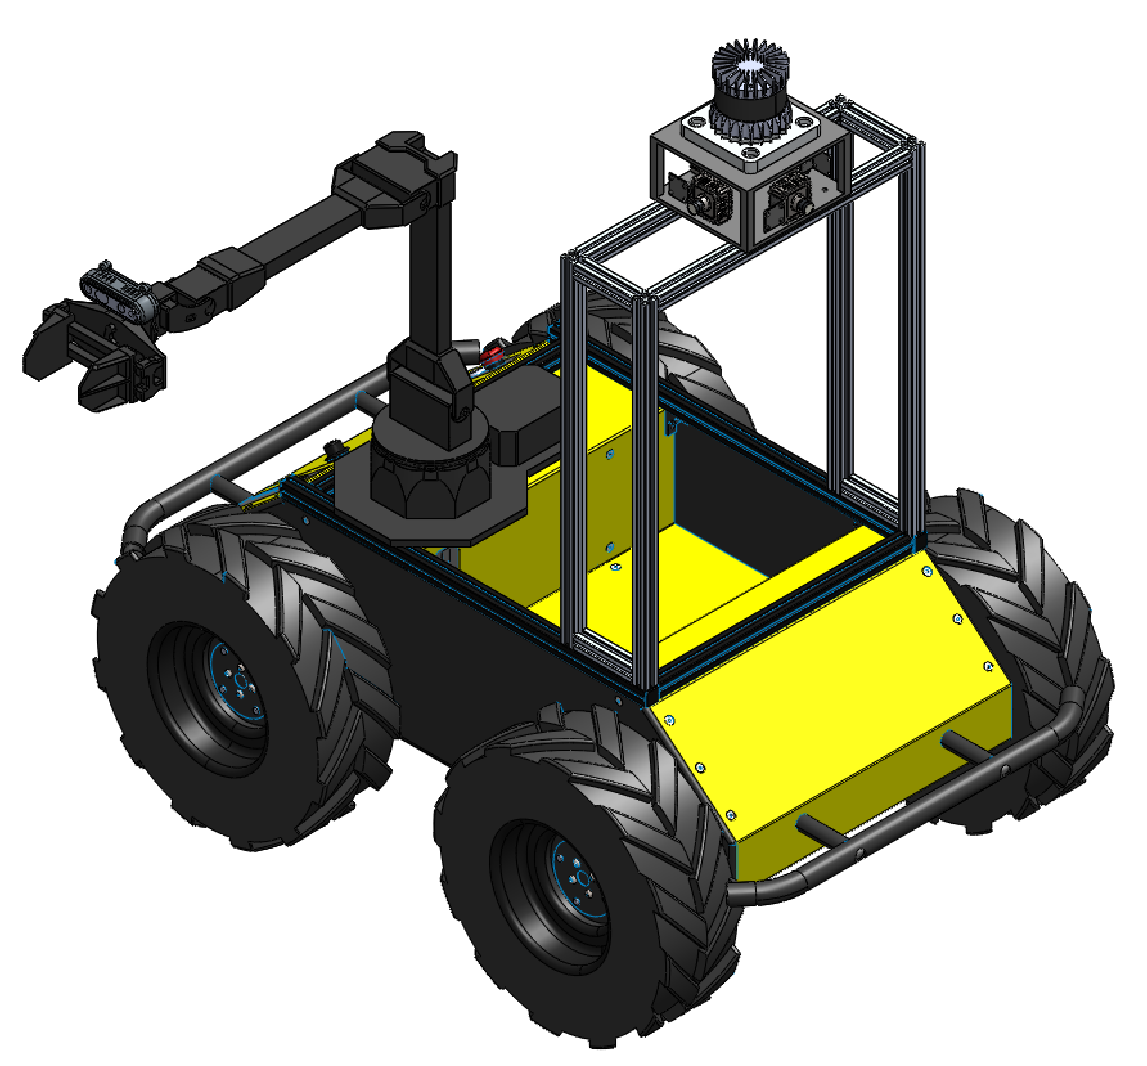
\includegraphics[width = 0.7\textwidth]{Figures/husky_completed.pdf}
  \caption{3D model of the complete robotic system.}
  \label{fig:hardware}
\end{figure}

\subsection{General Arrangement}
The UGV acts as a bracket that holds all sensors and actuators as well as having the role of powering all equipment it holds. A general arrangement drawing describing physical arrangement of all the components mounted on the UGV is presented in figure \ref{fig:general_arrangement}.

\begin{figure}[H]
  \centering
   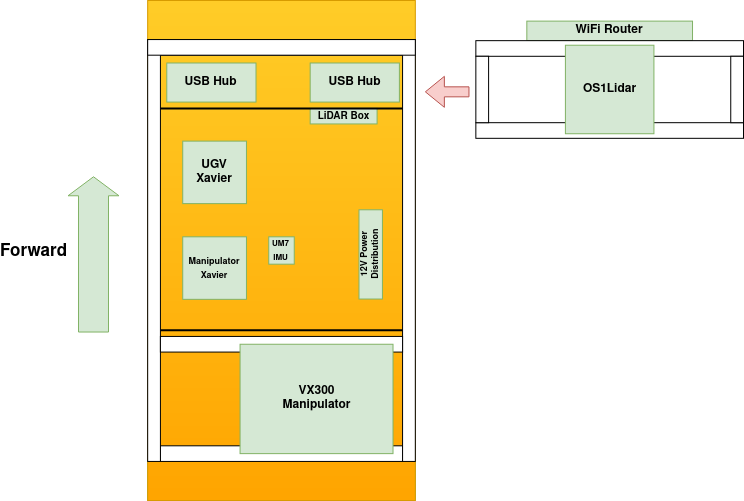
\includegraphics[width = 0.9\textwidth]{Figures/general_arrangement.drawio.png}
  \caption{General arrangement drawing of UGV platform. Here, the physical position of different hardware components are defined. The sensor frame is drawn to the left of the main frame.}
  \label{fig:general_arrangement}
\end{figure}

\subsection{Electrical Interface}
The different components in the system is powered through the user power supply of the UGV(see table \ref{tab:husky:a200:specs}). Figure \ref{fig:circuit_diagram} is a circuit diagram that illustrates the DC power distribution.

\begin{figure}[H]
  \centering
  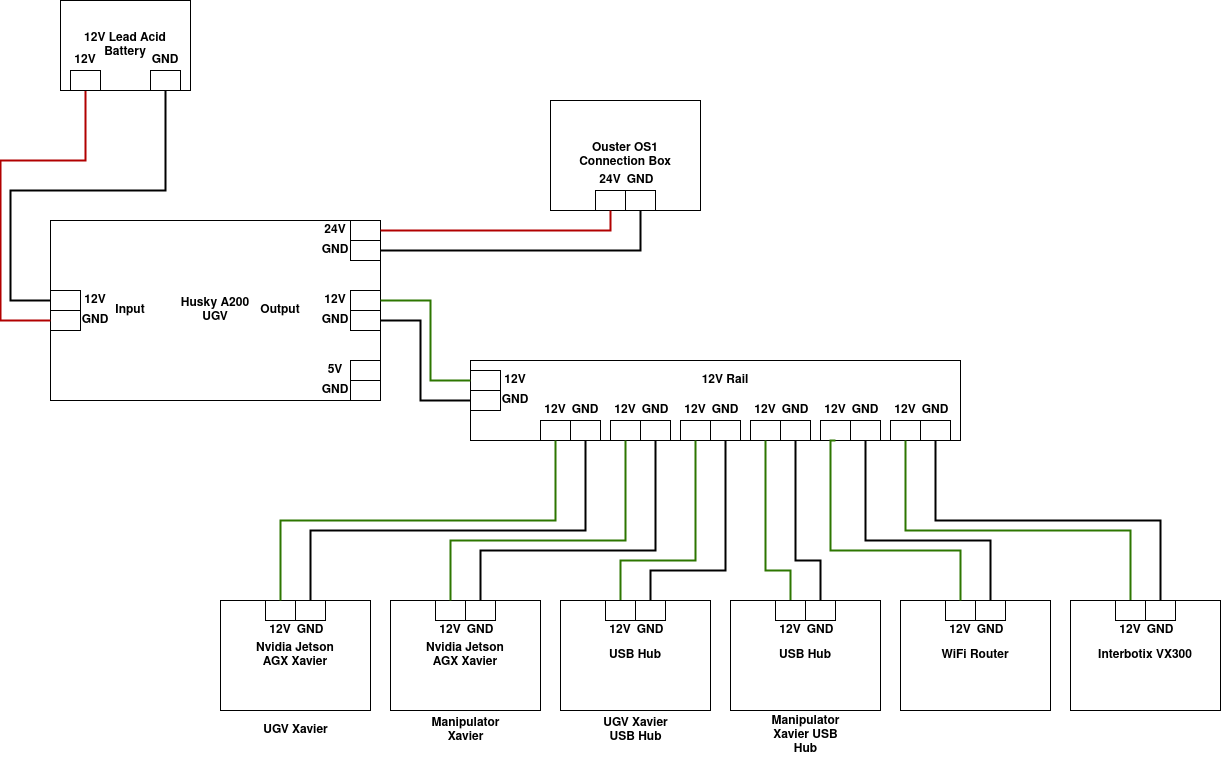
\includegraphics[width = 1\textwidth]{Figures/circuit_diagram.drawio.png}
  \caption{Circuit diagram showing the power distribution on the UGV}
  \label{fig:circuit_diagram}
\end{figure}

\section{Software Setup}
For the different components of the robotic system to act together, some software configuration has to be done. This section describes different  parts of the software setup to achieve an autonomously navigating robotic platform. As mentioned in \textbf{where i mention} ROS2 is used for software implementation. All ROS2 packages described in this section is either available as open source packages, or developed during the course of this project.

\subsection{UGV Setup}
\subsubsection{Husky ROS2 Packages}
An adaptation of Clearpath's own Husky A200 ROS2 packages are used to operate the UGV in ROS2. Clearpath husky provides Debian ROS2 packages for ROS2 Foxy, and these are therefore used. The story is different for ROS2 Galactic which has reached its EOL and is no longer maintained. Nevertheless, the official Husky ROS2 repository\cite{husky_repo} still contains a branch for ROS2 Galactic even though it won't build. This branch is forked and modified in order to build as well as modified to take in some arguments to the launch file. The forked repository is public and available at \cite{uia_husky_repo}.

The Husky ROS2 packages brings up the UGV and makes it ready to take velocity commands. The velocity commands are handled through the \lstinline{twist_mux} node. This node publishes velocity commands based on the incoming commands and the defined priority. The command is published to the \lstinline{/husky_velovity_controller/cmd_vel_unstamped} topic. Figure \ref{fig:rqt_husky} illustrates how the husky takes in velocity commands through that topic and then publishes the husky odometry through the \lstinline{/odom} topic. This odometry is then passed to the \lstinline{ekf_node} that also takes in IMU data from the UM7 IMU(\lstinline{/um7_driver}) and the OS1 LiDAR(\lstinline{ouster_driver}). The node \lstinline{ekf_node}, is an Extended Kalman Filter that fuses the odometry and IMU data in order to define the position of the robot \lstinline{base_link} relative to the \lstinline{/odom} transform.

\begin{figure}[H]
  \centering
  \includesvg[width = 0.9\textwidth]{Figures/husky_nodes.drawio.svg}
  \caption{RQT Node Graph of Husky running in ROS2 Foxy. In addition to the Husky ROS2 packages, \lstinline{um7_node}, \lstinline{ros2_ouster} and \lstinline{pointcloud_to_laserscan} is running.}
  \label{fig:rqt_husky}
\end{figure}

\subsubsection{Model Description}
In ROS2, urdf files are used to describe robotic systems. As extra hardware is mounted on the UGV, some extra urdf information has to be added in order to describe the spatial relationship between the UGV and accessories such as the LiDAR. This information is added in an own urdf file and passed upon launch of the husky.

A visual representation of the UGV with all accessories attached is preferable when interacting with the robot in rviz2. Meshes of the accessory frame with the LiDAR and LiDAR/camera mount is therefore generated and used in the urdf file for visaluzation. 



\subsection{IMU Setup}

\subsection{LiDAR Setup}

\subsection{IMU Fusion}

\subsection{Manipulator}
\subsubsection{Model Description}
\subsubsection{Panning Scene}

\subsection{Machine Vision}
\subsubsection{Camera Setup}
\subsubsection{Apriltag}


\section{Autonomous Navigation}
Autonomous navigation is achieved using the NAV2 navigation stack for ROS 2.

\subsection{SLAM}

\subsection{Navigation 2}



\section{Algorithms}

\subsection{Scene Geometry Publisher}

\subsection{Husky Pick and Place}


\subsection{Husky Master Node}
On a high level, the system is controlled by a ros node called "husky\_master". This node interacts with NAV2 and Moveit 2 to orchestrate an autonomous pick and place operation. The interaction between "husky\_master" and Moveit 2 is done through "husky\_pick\_and\_place" which acts as an interface between Moveit 2 and "husky\_master". A high level overview of this interaction is shown in figure \ref{fig:husky_master}

\begin{figure}[H]
  \centering
  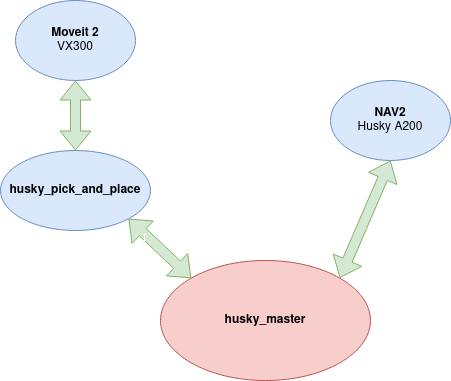
\includegraphics[width = 0.6\textwidth]{Figures/software_overview.drawio.png}
  \caption{The "husky\_master" node controls the operation by interfacing directly with NAV2 and with Moveit2 through the "husky\_pick\_and\_place" node.}
  \label{fig:husky_master}
\end{figure}
